% Drawing 144/06-2 -- folder 144, batch 06, archive page 104 (PDF page 105).
% Transcription: Un point base d'où partent des chemins vers les points $0$, $1/2$, $1$ d'une droite horizontale, chacun contournant le point par un petit lacet fléché ; plus loin sur la droite un point $z$ et, au bout, $\infty$.
% Kind: paths from a base point to 0, 1/2, 1, each turning round the point. Method 2 (schematic redraw from the facsimile). Status: ok.
% Notes: A base point on an upper horizontal line; three oriented paths from it go down to 0, 1/2, 1 on the lower line, each ending in a small loop round the point. Further on the lower line the point z; the end "infinity" is beyond the right edge of the crop. The labels 0, 1/2, 1 under the loops are as legible (the 1 is read from the transcription).
% Coordinates: 1 unit = 1 mm = 1/100 of the crop width (bbox in page fractions: [0.4, 0.08, 0.8, 0.24]).
% Redrawn by Claude (claude-opus-5-5), issue #73, 2026-11-07; not checked by a human; not compiled (no TeX in the session).
% Rights: reproduces part of the work -- behind RENDER_TRANSCRIPTS, never published by itself.
\documentclass[tikz,border=3pt]{standalone}
\usepackage{amsmath,amssymb}
\usetikzlibrary{patterns,arrows.meta}
\tikzset{pencil/.style={black!45}, struck/.style={black!35}, mark/.style={circle,draw,inner sep=1.3pt}, pt/.style={circle,fill,inner sep=0.9pt}, opt/.style={circle,draw,fill=white,inner sep=1.1pt}}
\begin{document}
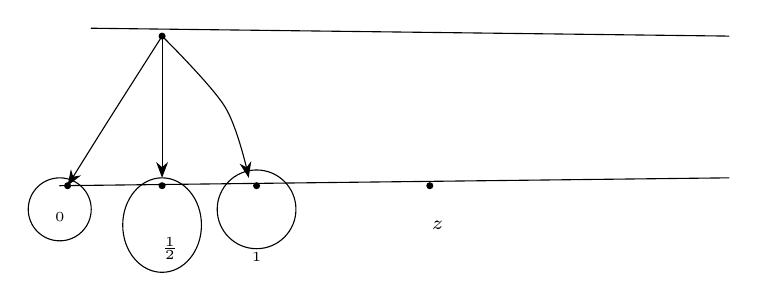
\begin{tikzpicture}[x=1mm,y=1mm,line cap=round,line join=round,font=\scriptsize]
\draw (14,-12) -- (95,-13);
\node[pt] at (23,-13) {};
\draw (10,-32) -- (95,-31);
\draw[-{Stealth[length=2mm]}] plot[smooth, tension=0.55] coordinates {(23,-13) (16,-24) (11,-32)};
\draw[-{Stealth[length=2mm]}] (23,-13) -- (23,-31);
\draw[-{Stealth[length=2mm]}] plot[smooth, tension=0.55] coordinates {(23,-13) (31,-22) (34,-31)};
\draw (10,-35) circle[radius=4];
\draw (23,-37) ellipse[x radius=5, y radius=6];
\draw (35,-35) circle[radius=5];
\node[pt] at (11,-32) {};
\node[pt] at (23,-32) {};
\node[pt] at (35,-32) {};
\node[pt] at (57,-32) {};
\node[inner sep=1pt] at (10,-36) {\tiny $0$};
\node[inner sep=1pt] at (24,-40) {\tiny $\tfrac12$};
\node[inner sep=1pt] at (35,-41) {\tiny $1$};
\node[inner sep=1pt] at (58,-37) {\scriptsize $z$};
\end{tikzpicture}
\end{document}
